\documentclass{report}

% Page layout
\usepackage{geometry}
\geometry{
	a4paper,
}

% Fonts
\usepackage{fontspec}
\defaultfontfeatures{Mapping=tex-text,Scale=MatchLowercase}
\setmainfont{Linux Libertine O}

% Language
\usepackage{polyglossia}
\setdefaultlanguage{english}

% Graphics
\usepackage{graphicx}
\graphicspath{{./images/}}

% Links
\usepackage{url,hyperref}

% Headers and footers
\usepackage{fancyhdr}
\pagestyle{fancy}
\fancyhf{}
\lhead{
\includegraphics[scale=0.1]{inp-enseeiht}}
\rhead{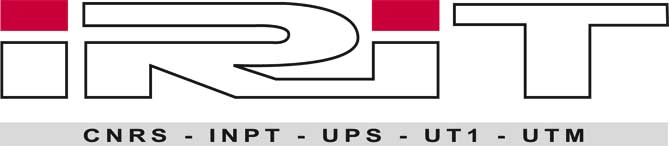
\includegraphics[scale=0.1]{irit}
\lfoot{Three-dimensional modeling and printing}}
\rfoot{\thepage}

% Code
%\usepackage{minted}

\begin{document}

\bigskip
\bigskip
\bigskip
\bigskip
\bigskip
\bigskip
\bigskip
\bigskip

\begin{center}
\huge{Three-dimensional modeling and printing:\\ Project report\\}
\bigskip
\bigskip
\Large{from January 23 to March 16, 2012}
\end{center}

\bigskip
\bigskip

\begin{center}
\large{
\textit{Vincent \textsc{Duvert} \\
Antoine \textsc{Lubineau} \\
Caroline \textsc{Naud} \\
James \textsc{Packer} \\
Florian \textsc{Ribon}} \\
\bigskip
INP-ENSEEIHT/IMA 
}
\end{center}

\bigskip
\bigskip

	This report summarizes the context, organization, work and outcomes within the 3D modeling and printing project suggested by the VORTEX team of IRIT to third-year students in the IMA department of ENSEEIHT.

\bigskip
\bigskip

\begin{figure}[!h]
\begin{center}
	
\includegraphics[scale=0.4]{inp-enseeiht}
\end{center}
\end{figure}

\bigskip

\begin{center}
\url{http://www.enseeiht.fr/fr/index.html} \\
2 Rue Charles Camichel \\
31 071 TOULOUSE
\end{center}

\vfill

\begin{figure}[!h]
\begin{center}
	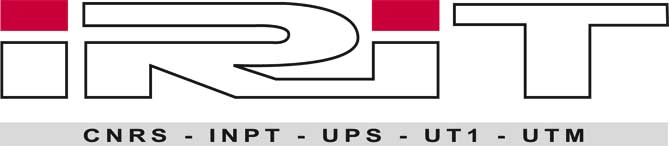
\includegraphics[scale=0.4]{irit}
\end{center}
\end{figure}

\begin{center}
\url{http://www.irit.fr}\\
Université Paul Sabatier \\
118 Route de Narbonne \\
F-31062 TOULOUSE CEDEX 9
\end{center}

\thispagestyle{empty}

\newpage

\chapter*{Acknowledgments}
\addcontentsline{toc}{chapter}{\numberline{}Acknowledgments}

	Our most sinceres thanks go to our technical supervisor, Lionel \textsc{Cremel}, for guiding us throughout this two-months project and having initiated us in a progressive and efficient way to the art that is project management. Our project would certainly not have got the same results without him.\\

\bigskip

	Therefore we want to thank Axel \textsc{Carlier}, Jean \textsc{Conter} and Géraldine \textsc{Morin} for having proposed us such an interesting subject and for all the help and the pieces of advice they have been giving us during the project.\\

\bigskip

	We also thank all the people we have met during our visits to the manufacturing laboratory \textsc{Artilect} who got interested in our project and agreed to share with us their expertise in this area.

\tableofcontents

\chapter{Presentation of the project}

\section{The context}

	The \textit{3D printing} phrase is used to describe the process of creating three dimensional objects from digital files using a materials printer in a manner similar to printing images on paper. The term is most closely associated with additive manufacturing technology, where an object is created by laying down successive layers of material.\\

	Since 2003 there has been a large growth in the sale of 3D printers since the technology actually finds use in more and more fields such as the fields of jewellery, footwear, industrial design, architecture, engineering and construction (AEC), automotive, aerospace, dental and medical industries, education, geographic information systems, civil engineering, and many others.\\

	The VORTEX team (Visual Objects : from Reality To EXpression) from IRIT (Institut de Recherche en Informatique de Toulouse) is part of the numerous people having found interest in this technology and recently acquired an Ultimaker 3D printer on which she has no control over yet and that she would like to be able to use in order to print 3D mono-color objects. To that end, she would need to be able to create, model and edit these objects within a software (to be conceived or modified) using, if possible, the multi-touch screen she already owns (Acer T231H).\\

\section{The final users of the product}

	The primary final users of the 3D modelling software and of the printer would be the researchers of the team of IRIT. However, they really aim at offering this service to artists, such as those already using an Ultimaker 3D printer in the Fablab in Toulouse.

\section{The work required}

	The project was divided into two major parts. The first consisted in developing an open-source software with graphical interface that could allow to model and deform virtual 3D objects, preferably using a dual-touch screen. The second part concerned the export of this object (as a mesh) to the printer to finally print it as realistically as possible.

\section{Available resources}

\subsection{The project team}

	Our team was composed of five students from the Computing and Applied Mathematics department of ENSEEIHT who all showed a real interest in the subject. These people are listed here:

\begin{itemize}
\item Caroline \textsc{NAUD}: project manager
\item Vincent \textsc{DUVERT}
\item Antoine \textsc{LUBINEAU}
\item James \textsc{PACKER}
\item Florian \textsc{RIBON}
\end{itemize}

\subsection{Material resources}

	We list below all the material resources which were available to us during the project:

\begin{itemize}
\item the room F117 in building F at ENSEEIHT (same building that the one the \textsc{VORTEX} team works in
\item an Ultimaker 3D printer with a roll of PLA plastic
\item a computer with a dual-touch screen Acer T231H
\item all computer rooms of ENSEEIHT
\item our personal computers
\end{itemize}

\chapter{Project management}

\section{Project supervision}

	During the first week of the project we were introduced to Lionel \textsc{Cremel}, project manager at \textsc{Airbus}, who had volunteered to guide us in managing our project. We agreed on that day to meet him at least once a week nearly every week so that he could guide us throughout the project. We give here the dates on which we successively met and the main content of the meeting:
	
\begin{itemize}
\item Week 1 (January, 24): introduction of the project members, choice of the project management model, introduction of the specification phase of the V model
\item Week 2 (January, 27): choice of the project manager, 
\item Week 3 (February, 6):
\item Week 4 (February, 9):
\item Week 5 (February, 20):
\item Week 6 (February, 29):
\item Week 7 (March, 8):
\item Week 8 (March, 14):
\end{itemize}

On each meeting, Lionel successively explained us how to decide of a macroscopic planning for our project, told us about the different milestone they use in Airbus projects and the documents that should sometimes be available when arriving at a milestone and guided us throughout the management of our human and material resources. Of course, we couldn't do exactly as he was used to doing in Airbus (simply because our project is happening in quite special conditions) but thanks to that, we could have a real idea of what project management would be in the future. 

\section{Resource management and planning}

With the help of Lionel, we all agreed on saying that a V-cycle was adequate for the progress of our project. This cycle includes (as shown on the picture below):

\begin{itemize}
\item a specification part (requirements, design and architecture) on which the final user tests and the functional tests are decided,
\item an implementation part on which unit tests are run on the different functionalities implemented,
\item a validation phase on which all the tests are run and at the end of which a final acceptance should be obtained from the client.
\end{itemize}

\begin{figure}[!h]
\begin{center}
	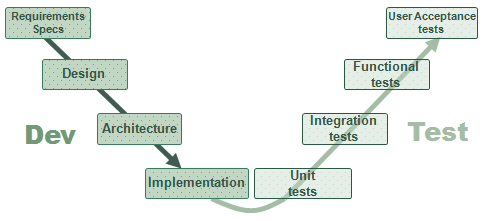
\includegraphics[scale=4.5]{VCycle}
\end{center}
\end{figure}

However, our project was special an could not totally follow that scheme since it contained a part on which we had to learn how to use the printer and which were the adapted parameters to get good quality objects. We thus thought that this part deserved to have at least one member of the team dedicated to it at full time. This member would of course participate in the rest of the project but would spend most of his time on the printer. The four other members would equally participate in all the different steps of the project. Three of us would use their personal computers while the last one would sometimes work from his place or from the computer room at ENSEEIHT and would sometimes use the computer made available to us by the client team. This last one would also often be used by the student dealing with the printer to pilot it.\\\\

The macroscopic planning we chose is given here:

\bigskip
\begin{figure}[!h]
\begin{center}
	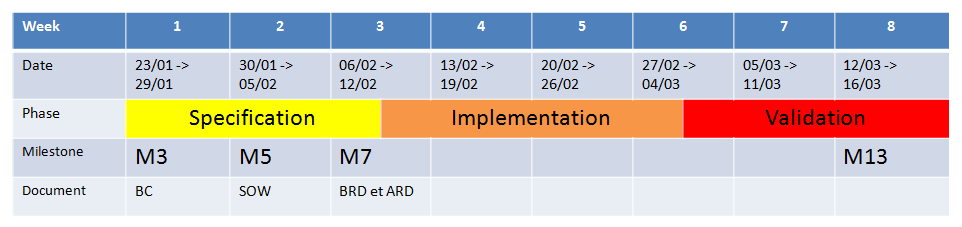
\includegraphics[scale=0.4]{PlanningMacroscopique}
\end{center}
\end{figure}

As shown here, we decided to give approximatively the same time to each mail part of our project, this is to say 2 to 3 weeks. The first main phase is here the only one containing milestones. This is because these were quite the most important milestones to us. They corresponded to the main documents we had to produce before starting the development. These documents will be given later in this report. They had to be submitted to the client so that we would be totally sure that we add completely understood their need. \\

A more detailed planning containing the different tasks we achieved is available in the appendix and will be explained in the rest of this report.

\section{The risks assessment}

Our supervisor also taught us how to manage the possible risks in our project so that we would not have any delay of major issues which would prevent us from delivering a good quality product. This work included the detection of theses risks, the finding of a way to prevent them and of a way to correct them if they would still happen. Of course, this assessment changed as time went by since some of the risks disappeared or actually happened and new appeared.

We give here an example of this assessment we did on our second week of work:

\bigskip
-- first risks assessment
\bigskip

\chapter{The specification phase}

This was the first main phase of our project. Our main goal at the end of this phase (--date'--)  was to fully determine with the client the specifications of the project so that we would change them as little as possible. The achievement  of this goal included to first understand what the client team expected from us on a general way (Statement Of Work) to them detail these needs and find technical solutions to satisfy them. This phase thus implied regular meetings with the client team.

\section{The establishment of the Statement Of Work}

We first met the client team on --date-- when they completely presented us the project for the first time. One of us was missing that day because still in semester abroad but we managed to tell him all about that meeting afterwards. \\

The client team first told us about this Ultimaker 3D printer she recently acquired and on which she had still no control over. Our main goal was ...

\section{The general architecture of the project}

As we all started to discover the printer, it came to us that the final application would include the use of several software. Indeed, the use of the printer first implies the transformation of the mesh created with the modeller into instructions for the printer (GCode) which we then need to send to the printer previously parametrized. This makes the 4 main parts given in the following figure:

\begin{figure}[!h]
\begin{center}
	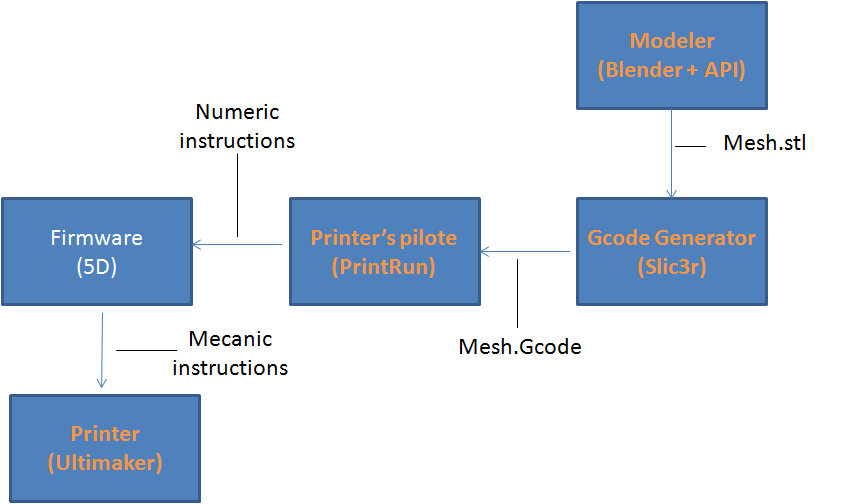
\includegraphics[scale=0.2]{ARD1}
\end{center}
\end{figure}

The terms written in orange are the only one we decided to act on. The printer's firmware could actually be replaced by some others but we decided that this was not necessary and that we would rather focus on the modeller, Gcode generator and printer's pilote. These choice of these is explained later in this report. 

\section{The redaction of the technical specifications}

One we had determined the clients' needs, we had to

\section{The technical choices}

\chapter{The implementation phase}

\section{The mesh correction - \textit{Florian \& James}}

We have implemented a script which allows the user to track broken, non-manifold edges on the working object in Blender, and offers him two different ways to correct them.

First of all, a press on the Check button highlights all the potential non-manifold edges and gives to the user the possibility to repair them if the mesh is actually non-manifold.

The first method is a soft correction algorithm, which detects all distincts holes in the mesh, then cleans theses holes (for instance if there are some faces not connected to any vertex), and finally try to fill them, each one after each one. This method is considered non-destructive (even if the cleaning part may remove unwanted faces) and is not recursive. The algorithm has been proven to make a broken mesh watertight, so there is no more holes remaining after its execution.

But even if it is watertight, a mesh may still remain non-manifold. Therefore, we implemented a strong correction algorithm which is able to repair all kinds of edges-related problems. This strong destructive method consists in a loop of soft correction calls, with a selection and removal of remaining non manifold edges (and thus which didn't belong to any standard hole) between each iteration. By properly removing these edges, new holes appear and the next iteration will try to fill them the correct way. Eventually, the mesh is fully manifold (thus watertight).

Both for the destructive method and the non-destructive one, we added a fast-processing option which makes the correction algorithms way faster than without enabling it. But activating it may results in various artifacts between some edges. Since it works better on bigger and well-detailed objects (with finer meshes), the user should try to use it first on big objects and if the result is not satisfying, he simply have to cancel the last operations then try again with fast-processing disabled. This option only acts during the holes filling action, by trying to fill all of them with only one single filling call, while the standard option requires another algorithm which we developed which detects and separates all distinct holes within the mesh.


\section{The choice of the supporting plane - \textit{Antoine \& Vincent}}

\section{The interface - \textit{Caroline}}

Although we had decided to work on Blender, its graphic interface remained quite difficult to use for inexperienced users and still showed ``useless'' functions. \\
While making researches about Blender, we discovered that we could manipulate its graphic interface as we wanted to only keep the most useful features visible. This was done while drag 	and dropping some windows and panels. We then registered the corresponding file (\textit{startup.blend}) to had it to the adequate place in the final product. We give here the original interface and the one we configured:

\bigskip

\begin{figure}[!h]
\begin{center}
	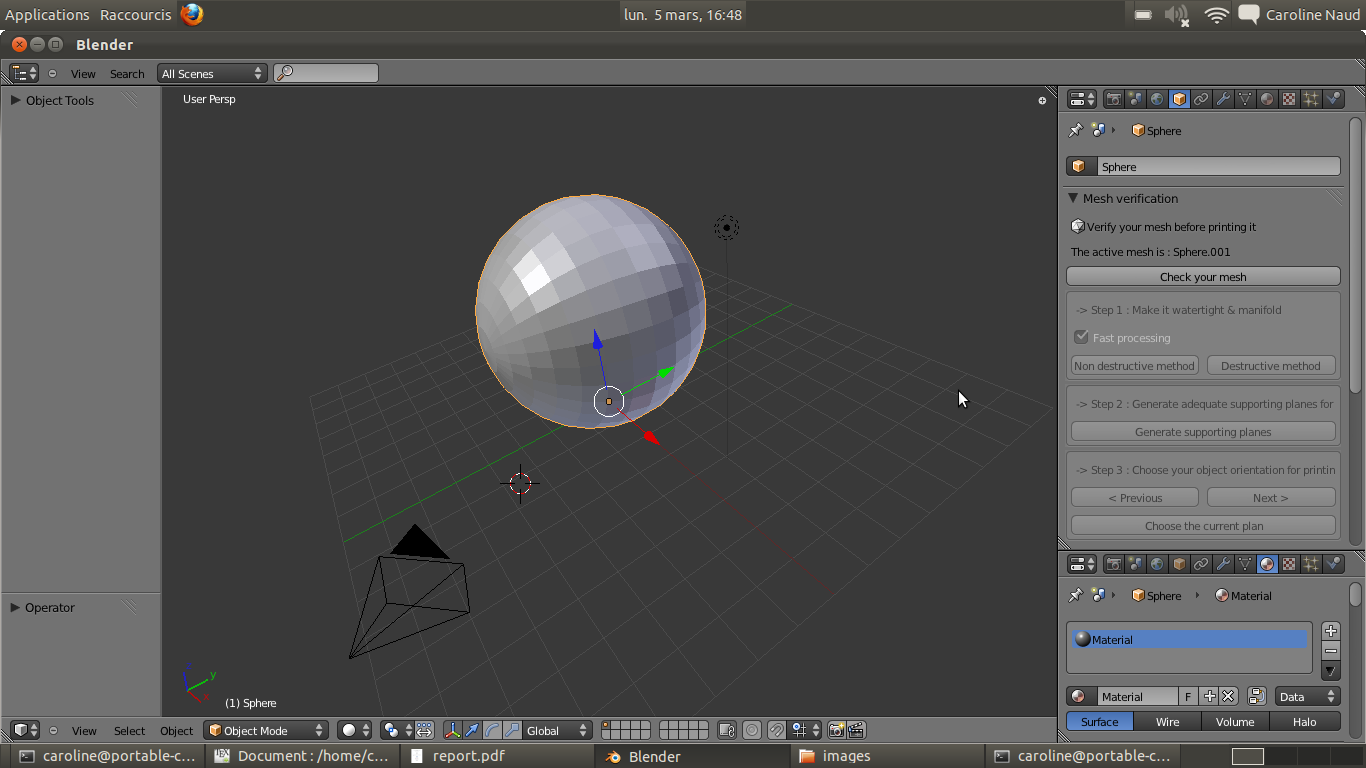
\includegraphics[scale=0.25]{NotreInterface}
\end{center}
\end{figure}

The part we see circled with red is the panel we added so that the user can have access to the different functions we implemented. It was also coded thanks to the Blender Python API which allows to create buttons, check boxes ... The panel is visible here:

\bigskip
--mettre le panneau--
\bigskip

As for the organization of the panel, we chose to divide if into 4 main parts that we called ``steps'' since we considered that the the user would have to use them successively. We detail these steps here below:

\begin{itemize}
\item Step 0: gives the user the current mesh's name and allow to check if the mesh is correct for printing (manifold and watertight)
\item Step 1: allow the user to correct the mesh
\item Step 2: allow the user to find the most adequate supporting planes for the object
\item Step 3: allow the user to visualize all the planes generated and to choose the one he prefers
\end{itemize}

\chapter{The printer calibration}

\chapter{The validation phase}

\section{Unit tests}

\section{Integration tests}

\section{Functional tests}

\section{User tests}

\addcontentsline{toc}{chapter}{\numberline{}Bibliography}

\appendix

\end{document}
